% Options for packages loaded elsewhere
\PassOptionsToPackage{unicode}{hyperref}
\PassOptionsToPackage{hyphens}{url}
%
\documentclass[
]{article}
\title{Relatório - Covid}
\author{Geovanna Favilla}
\date{14/03/2022}

\usepackage{amsmath,amssymb}
\usepackage{lmodern}
\usepackage{iftex}
\ifPDFTeX
  \usepackage[T1]{fontenc}
  \usepackage[utf8]{inputenc}
  \usepackage{textcomp} % provide euro and other symbols
\else % if luatex or xetex
  \usepackage{unicode-math}
  \defaultfontfeatures{Scale=MatchLowercase}
  \defaultfontfeatures[\rmfamily]{Ligatures=TeX,Scale=1}
\fi
% Use upquote if available, for straight quotes in verbatim environments
\IfFileExists{upquote.sty}{\usepackage{upquote}}{}
\IfFileExists{microtype.sty}{% use microtype if available
  \usepackage[]{microtype}
  \UseMicrotypeSet[protrusion]{basicmath} % disable protrusion for tt fonts
}{}
\makeatletter
\@ifundefined{KOMAClassName}{% if non-KOMA class
  \IfFileExists{parskip.sty}{%
    \usepackage{parskip}
  }{% else
    \setlength{\parindent}{0pt}
    \setlength{\parskip}{6pt plus 2pt minus 1pt}}
}{% if KOMA class
  \KOMAoptions{parskip=half}}
\makeatother
\usepackage{xcolor}
\IfFileExists{xurl.sty}{\usepackage{xurl}}{} % add URL line breaks if available
\IfFileExists{bookmark.sty}{\usepackage{bookmark}}{\usepackage{hyperref}}
\hypersetup{
  pdftitle={Relatório - Covid},
  pdfauthor={Geovanna Favilla},
  hidelinks,
  pdfcreator={LaTeX via pandoc}}
\urlstyle{same} % disable monospaced font for URLs
\usepackage[margin=1in]{geometry}
\usepackage{graphicx}
\makeatletter
\def\maxwidth{\ifdim\Gin@nat@width>\linewidth\linewidth\else\Gin@nat@width\fi}
\def\maxheight{\ifdim\Gin@nat@height>\textheight\textheight\else\Gin@nat@height\fi}
\makeatother
% Scale images if necessary, so that they will not overflow the page
% margins by default, and it is still possible to overwrite the defaults
% using explicit options in \includegraphics[width, height, ...]{}
\setkeys{Gin}{width=\maxwidth,height=\maxheight,keepaspectratio}
% Set default figure placement to htbp
\makeatletter
\def\fps@figure{htbp}
\makeatother
\setlength{\emergencystretch}{3em} % prevent overfull lines
\providecommand{\tightlist}{%
  \setlength{\itemsep}{0pt}\setlength{\parskip}{0pt}}
\setcounter{secnumdepth}{-\maxdimen} % remove section numbering
\ifLuaTeX
  \usepackage{selnolig}  % disable illegal ligatures
\fi

\begin{document}
\maketitle

\hypertarget{introduuxe7uxe3o}{%
\subsection{1 - Introdução}\label{introduuxe7uxe3o}}

Resultado da análise estatística básica sobre os efeitos da pandemia do
novo corona vírus. Os dados foram coletados a partir do sistema público
de saúde de Bauru - SP

\hypertarget{anuxe1lise-inicial}{%
\subsection{2 - Análise Inicial}\label{anuxe1lise-inicial}}

Para analisar a frequencia em que cada grupo etário era acometido pela
nova doença, um histograma foi gerado. Assim, é possível comunicar
visualmente com maior facilidade os grupos mais afetados na região.

\begin{figure}
\centering
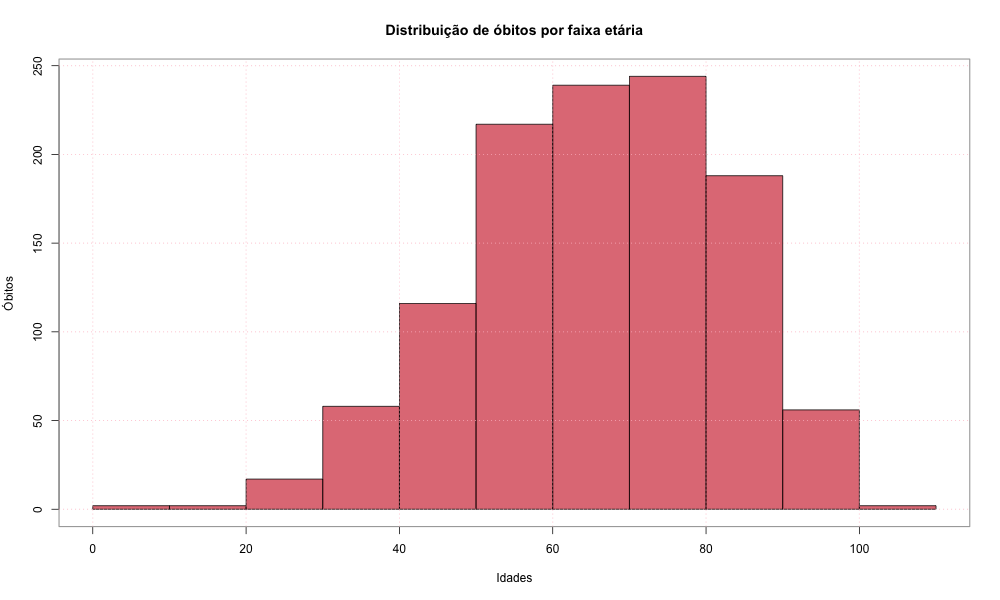
\includegraphics{/Users/Geovanna Favilla/Documents/UNESP/iead2021/tf-geovanna-favilla/graficos/idade-fig1.png}
\caption{Histograma - faixa etárias}
\end{figure}

É possível também analisar a média - em dias - de hospitalização,
separando os dados entre origem pública e privada:

\begin{figure}
\centering
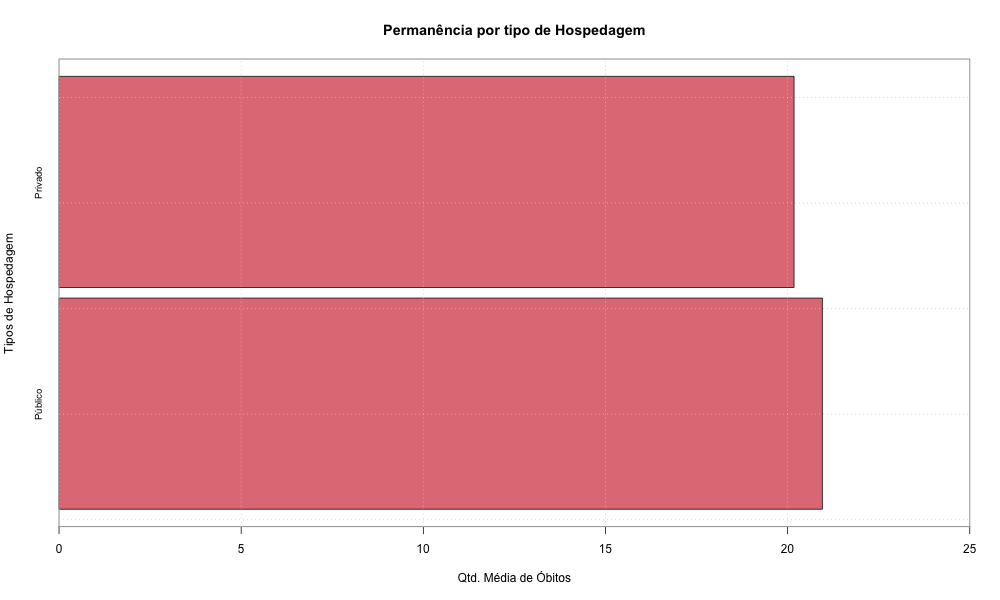
\includegraphics{/Users/Geovanna Favilla/Documents/UNESP/iead2021/tf-geovanna-favilla/graficos/internacao-fig1.png}
\caption{Gráfico 01 - Média de internação}
\end{figure}

É possível analisar, ainda que parcialmente, o número de óbitos
ocorridos durante o período amostrado:

\begin{figure}
\centering
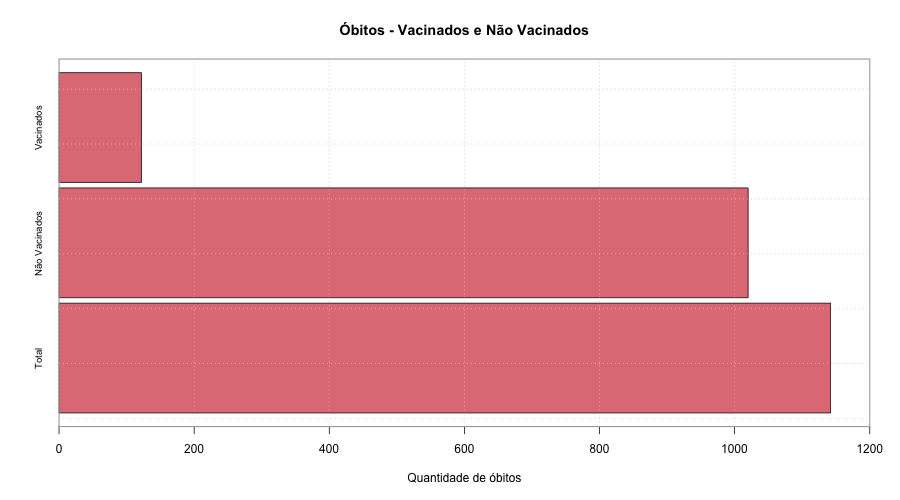
\includegraphics{/Users/Geovanna Favilla/Documents/UNESP/iead2021/tf-geovanna-favilla/graficos/obitos-vacinas.png}
\caption{Gráfico 02 - Óbitos}
\end{figure}

Outro aspecto importante (e muito discutido) na análise do background de
cada paciente são as comorbidades pré-existentes. A partir dos dados
fornecidos, é possível visualizar o panorama básico da região da cidade
de Bauru no que toca a esse assunto:

\begin{figure}
\centering
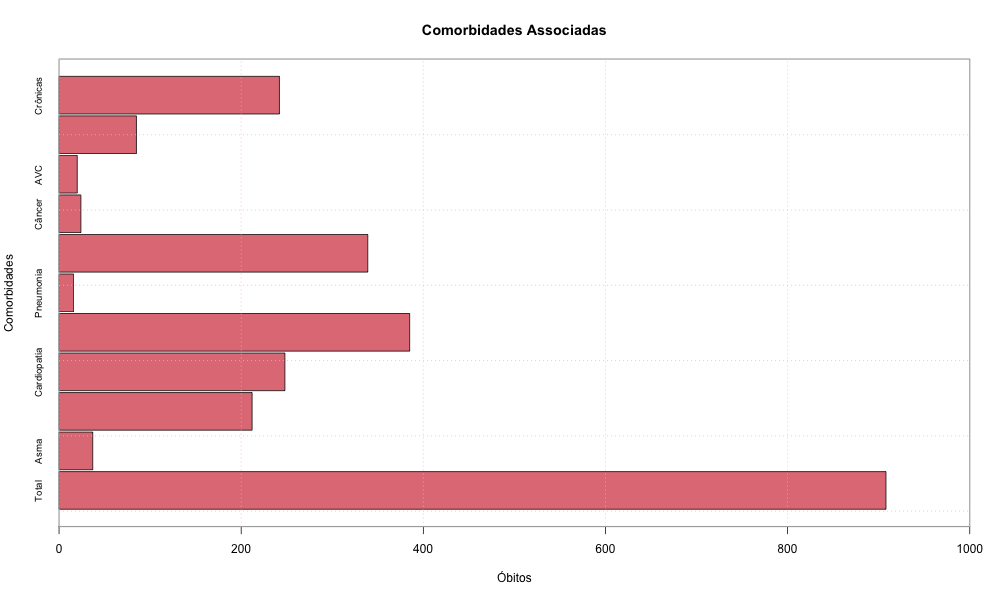
\includegraphics{/Users/Geovanna Favilla/Documents/UNESP/iead2021/tf-geovanna-favilla/graficos/comorbidade-fig1.png}
\caption{Gráfico 03 - Comorbidades Associadas}
\end{figure}

Por fim, uma análise superficial da evolução de óbitos durante a parte
mais crítica da pandemia. Podemos notar a acentuação e o crescimento da
curva de óbitos durante o referido período:

\begin{figure}
\centering
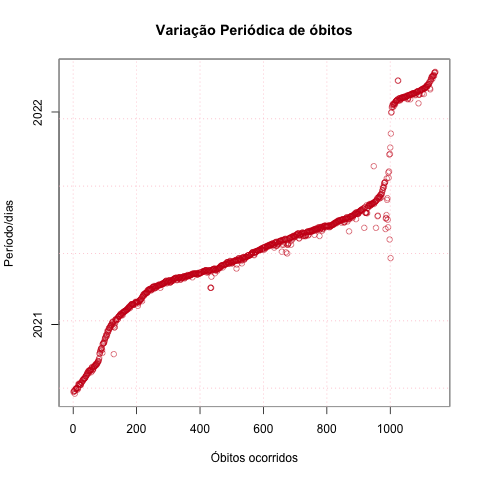
\includegraphics{/Users/Geovanna Favilla/Documents/UNESP/iead2021/tf-geovanna-favilla/graficos/varperiod-fig1.png}
\caption{Gráfico 04 - Variação de óbitos durante período crítico}
\end{figure}

\end{document}
